\begin{center}
\begin{table}[H]
\footnotesize
\centering
\begin{tabular}{ p{2.2cm} p{2.2cm} p{2.3cm} p{1.5cm} p{2.3cm} p{2.3cm}} 
\hline
Simulator & Implementation Language & Supported OS & Licence & Developer & High-Level Dependencies\\
\hline
Gazebo \cite{Koenig2005DesignSimulator} & C++ & Linux, MacOS & Apache V2.0 & Open Source Robotics Foundation & \\
\\
AirSim \cite{Shah2017AirSim:Vehicles} & C++ & Windows, Linux & MIT & Microsoft & Unreal Engine 4\\ 
\\
jMAVSim \cite{jMAVSim} & Java & Linux, MacOS, Windows & BSD 3 & DroneCode Project & Java3D\\
\\
HackFlightSim (renamed MulticoptorSim) \cite{MulticopterSim} & C++ & Linux, Windows & GPL & Simon Levy & Unreal Engine 4 \\
\\
RotorS \cite{RotorS} & C++ & Ubuntu & ASL 2.0 & ETH Zurich & ROS, Gazebo\\
\\
Morse \cite{Echeverria2011ModularMORSE} & Python & Linux & BSD & LAAS-CNRS & Blender Game Engine \\
\\
New Paparazzi Simulator \cite{Hattenberger2014UsingResearch} & C & Linux, MacOS & GPL v2 & Ecole Nationale de l’ Aviation Civil & JSBSim\\
\hline
\end{tabular}
\caption{Simulator Comparisons, based on \cite{Ebeid2018ASimulators}}
\label{table:SimulatorComparison}
\end{table}
\end{center}
In order to add high-level autonomous aerial vehicle support to the simulation environment, we used the AirSim \cite{Shah2017AirSim:Vehicles} plugin for UE4. Table \ref{table:SimulatorComparison} shows candidates that were considered to provide the support for simulated RAVs. We chose to use AirSim with UE4 over other simulation technologies for the following reasons, based on the paper published by the AirSim team \cite{Shah2017AirSim:Vehicles}:

\begin{itemize}
\item The design process of the physical environment could be decoupled from the plugin and other plugins could add further functionality independently of AirSim. This meant that new versions of AirSim could be seamlessly integrated with the existing simulation.

\item UE4 has ample documentation and is highly suited to simulating physical phenomena.

\item AirSim has high-level, extensible navigation and sensor APIs for multiple programming languages.

\item AirSim provides the ability to run multiple RAVs and RGVs in the same environment.

\item AirSim has been open-sourced with an MIT licence and was designed to be easily extended.

\item AirSim  provides an API to render unmodified images, depth maps and segmented images.

\item AirSim is highly modular in its approach to modelling sensors and actuators, which means that it can easily be extended with domain-specific functionality.

\item AirSim supports flight controller firmware such as PX4, ROSFlight and Hackflight with minimal setup.

\end{itemize}
AirSim internally models RAVs using different low-level modules outlined in \cite{Shah2017AirSim:Vehicles}. Figure  \ref{fig:AirSimArchitecture}, published in \cite{Shah2017AirSim:Vehicles}, provides an overview of how the different components of the simulator work together.

\begin{figure}[H]
    \centering
    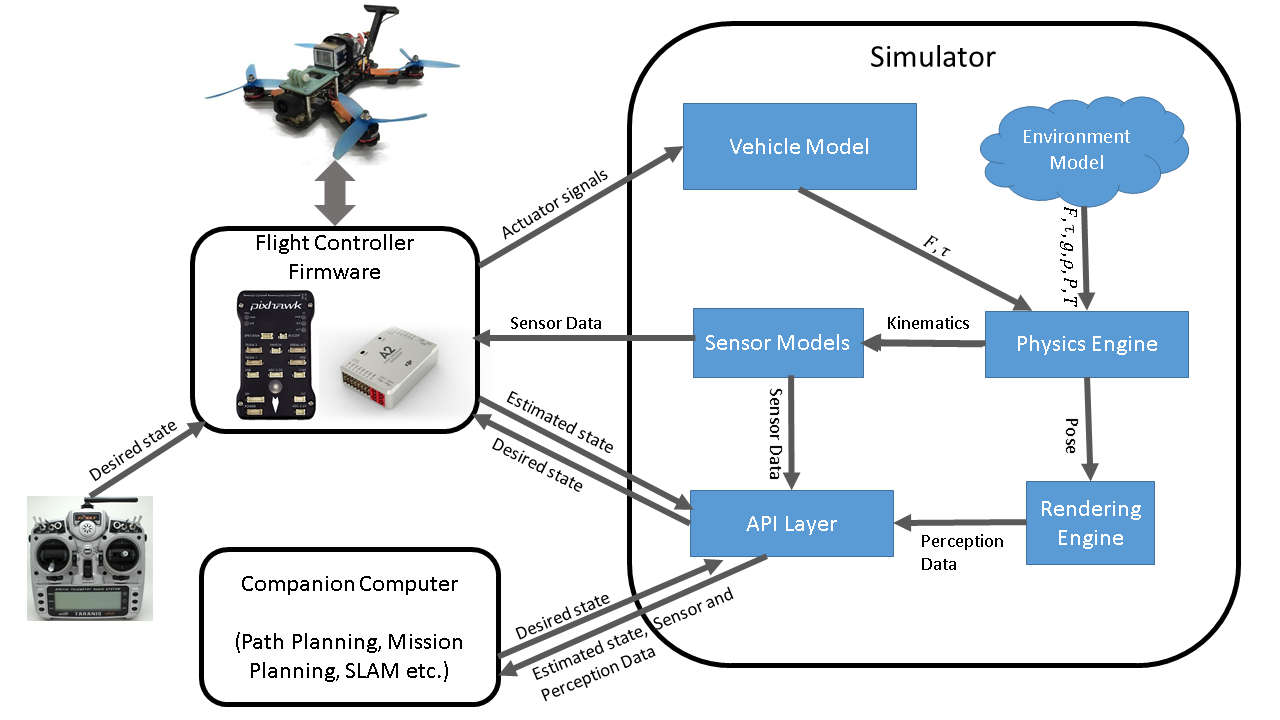
\includegraphics[width=0.75\linewidth]{Chapters/SimulationEnv/Figs/AirSimArchitecture/AirSimArchitecture.png}
    \caption{The architecture of the AirSim simulator. Diagram taken from \cite{Shah2017AirSim:Vehicles}}
    \label{fig:AirSimArchitecture}
\end{figure}



%Details of how to integrate AirSim into a custom UE4 project can be found %https://microsoft.github.io/AirSim/docs/unreal_custenv/.
%\note{It might be worth discussing how airsim actually models the state of the drone and its ability to integrate with PX4 over mavlink}. 
%\note{Discuss how the API works in order to achieve high-level tasks.}
Once the plugin had been successfully integrated into the project, some additional functionality was added to meet some of the design objectives, described in the subsequent section.

\subsection{Modifications and Extensions}
\note{Debugging lines added to API, additional cameras added, Radiation simulator and simulated detector added, battery simulator added, on-screen debugging messages added, GPS-to-NED conversion tools, debugging lines to show where drones have gone as well as planned routes.}

As shown in Figure \ref{fig:AirSimArchitecture}, AirSim maintains the internal state related to the vehicles that it is simulating and allows the user to modify this state through an API layer. In practice, this means that adding functionality to the API layer involves modifying a number of layers underneath the API layer. 
%The repository developers published some guidelines on how to modify the code, which can be found here: (in comment). %https://microsoft.github.io/AirSim/docs/dev_workflow/. 
While making all the changes listed below, the steps
\href{https://microsoft.github.io/AirSim/docs/dev\_workflow/}{documented by the plugin authors}\footnote{\href{https://microsoft.github.io/AirSim/docs/dev\_workflow/}{https://microsoft.github.io/AirSim/docs/dev\_workflow/}}
were followed: first, the plugin code is edited in order to add the desired functionality, then the plugin is built, added to a UE4 environment and tested. This process is necessary since AirSim is a plugin - there is no easy way to run and test it as a standalone piece of code. All of the modifications were made to a fork of the \href{https://github.com/microsoft/AirSim}{main AirSim repository}\footnote{\href{https://github.com/microsoft/AirSim}{https://github.com/microsoft/AirSim}}.
%\note{Add quick overview of RPC and how API works generally}

\subsubsection{AirSim API Overview}
In order to make modifications to the AirSim API, it is necessary to understand how the API has been designed. The API is socket-based over \href{http://rpclib.net/}{rpclib}\footnote{\href{http://rpclib.net/}{http://rpclib.net/}}, a library that implements the \textbf{R}emote \textbf{P}rocedure \textbf{C}all (RPC) using the \href{https://msgpack.org/}{msgpack}\footnote{\href{https://msgpack.org/}{https://msgpack.org/}} binary serialization protocol for speed. The server contains an instance of the RPC server, and binds methods exposed to the user to internal methods responsible for interacting with the simulation. The server effectively dispatches the user's request to internal API's that are not directly exposed to the user, which are responsible for modifying the simulation parameters as the simulation proceeds.

The RPCLibServerBase class uses the \textbf{P}ointer to \textbf{Impl}ementation (PImpl) design to bind the RPC server to an instance of the ApiProvider class, which is responsible for dispatching commands to the three base class defining internal APIs that are currently implemented in AirSim:
\begin{itemize}
    \item VehicleApiBase, which is responsible for getting the state from the vehicle and sending controls commands to the vehicle. Derived classes define additional methods specific to a vehicle.
    \item VehicleSimApiBase, which is responsible for handling commands that aren't directly related to the vehicle's state, such as rendering the vehicle in UE4.
    \item WorldSimApiBase, which handles non-vehicle specific commands, for example setting the time of day in the simulation.
\end{itemize}

%\note{A diagram would probably help here, it's more complicated than it sounds.}

\subsubsection{Debugging Lines for Planned Routes}
%\note{Not sure if this is worth talking about - it was a complex process but can be summarized very well in a few lines}

\begin{wrapfigure}{r}{0.65\textwidth}
    \centering
    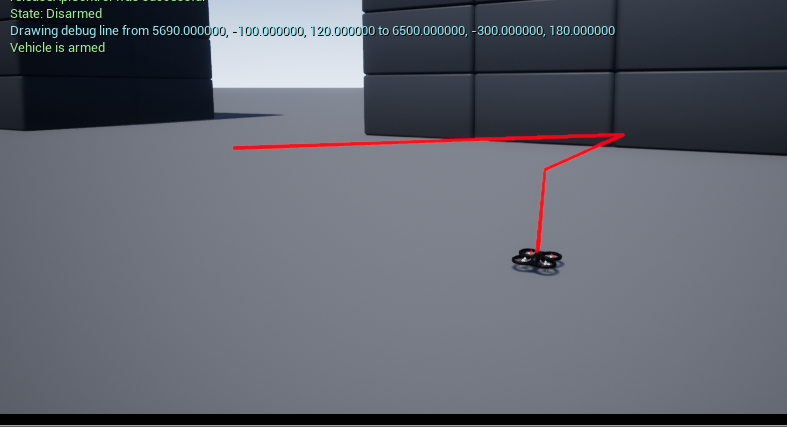
\includegraphics[width=0.65\textwidth]{Chapters/SimulationEnv/Figs/DebuggingLines/DebugLines.png}
    \caption{Debugging Lines Visualise planned RAV route.}
    \label{fig:DebuggingLines}

    \centering
    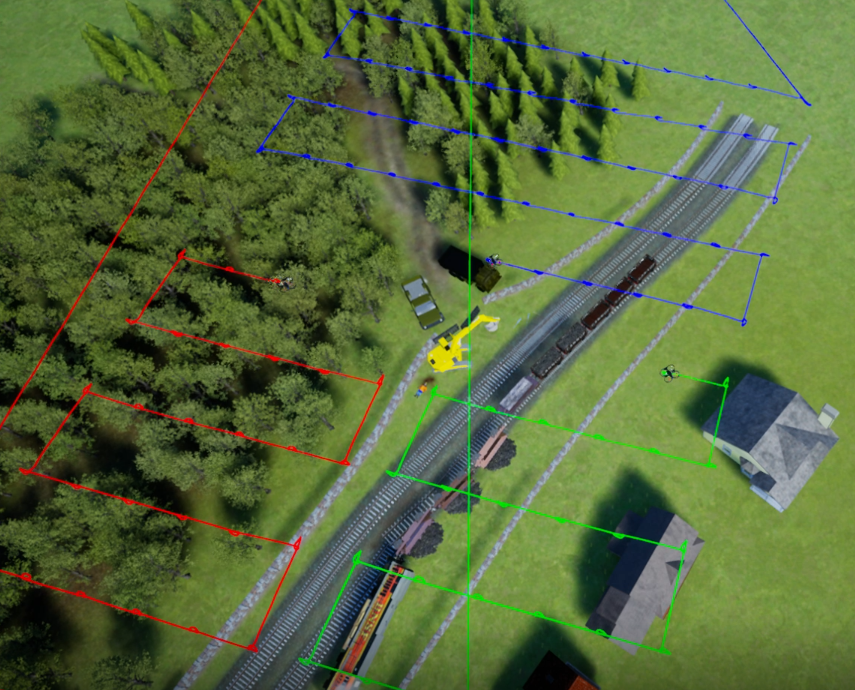
\includegraphics[width=0.65\textwidth]{Chapters/SimulationEnv/Figs/DebuggingLines/RoutesWithRAVsVisible.png}
    \caption{RAV path visualised mid-way through planned mission.}
    \label{fig:DebuggingLinesPlannedMission}
\end{wrapfigure}
The first modification made to AirSim was to extend the API to allow the user to visualize planned routes using debugging lines. %This functionality had already been requested on the repository page and since we also wanted the functionality, we decided to add this to the AirSim API. 
The end result can be seen in Figure \ref{fig:DebuggingLines}. We used a top-down approach to make the appropriate changes. First, we specified the functionality that we wanted to expose through the AirSim API. This was determined to be as follows: given 2 points in the 3-Dimensional Unreal Engine Frame of Reference (NED), a line thickness, a line colour and a time which the line will be shown for, display the specified line in the simulation environment. We wanted this to be available in both the global frame of reference and the local RAV frame of reference. This was planned to allow the user to visualise a series of lines from one specified waypoint to the next, on aggregate creating a visualisation of a planned path.
\newline


First, the methods simShowDebugLines and showPlannedWaypoints were added to the client code, in RpcLibClientBase.hpp, with method signatures
\begin{verbatim}
void simShowDebugLines(double x1, 
    double y1,
    double z1,
    double x2,
    double y2,
    double z2,
    double thickness, 
    double lifetime,
    const std::string& debug_line_color
);
\end{verbatim}
\begin{verbatim}
void showPlannedWaypoints(double x1, 
    double y1, 
    double z1, 
    double x2, 
    double y2, 
    double z2, 
    double thickness, 
    double lifetime,
    const std::string& debug_line_color,
    const std::string& vehicle_name = ""
);
\end{verbatim}

The corresponding server methods were added to RpcLibServerBase.cpp with the following signatures:
\begin{verbatim}
pimpl_->server.bind("simShowDebugLines", [&](double x1,
double y1, double z1, double x2, double y2, double z2,
double thickness, double lifetime, 
const std::string debug_line_color) -> void {
        getWorldSimApi()->showDebugLine(x1, y1, z1, x2, y2, z2, 
        thickness, lifetime, debug_line_color);
});
\end{verbatim}
%//vector<Vector3r> conv_path;
%//RpcLibAdapatorsBase::to(path, conv_path);
		

\begin{verbatim}
pimpl_->server.bind("simShowPlannedWaypoints", [&](double x1, 
    double y1, double z1, double x2, double y2, double z2, 
    double thickness, double lifetime, 
    const std::string debug_line_color,
    const std::string& vehicle_name) -> void {
            getVehicleSimApi(vehicle_name)->showPlannedWaypoints(x1, 
            y1, z1, x2,y2, z2, thickness, lifetime, 
            debug_line_color);
});
\end{verbatim}

The server delegates the handling of the debug line display to the worldSimApi in the case that the user wants to display in the global reference frame in the first case and the vehicleSimApi handles the local reference frame in the second case. 

A concrete implementation of vehicleSimApi then transforms the coordinates to the local reference frame of the vehicle. The showDebugLine method added to AirBlueprintLib.cpp uses the DrawDebugLine method, defined in the DrawDebugHelpers library, to directly interface with UE4 to draw the debug lines.

\begin{verbatim}
void DrawDebugLine
(
    const UWorld * InWorld,
    FVector const & LineStart,
    FVector const & LineEnd,
    FColor const & Color,
    bool bPersistentLines,
    float LifeTime,
    uint8 DepthPriority,
    float Thickness
)
\end{verbatim}
\par


Debug lines showing where the RAV has travelled were also added to the simulation. This was done by using a Blueprint, outlined in section \ref{subsubsec:blueprints}. A variable, $oldPos$, is used to store the previous position of the RAV. Every 0.2 seconds, the position is updated and a line is drawn from the RAV's old position to its new position. The user has the option to turn debugging lines on or off by setting a binary variable in the blueprint.

\note{Might be better to have this wrapfigure}
\begin{figure}
    \centering
    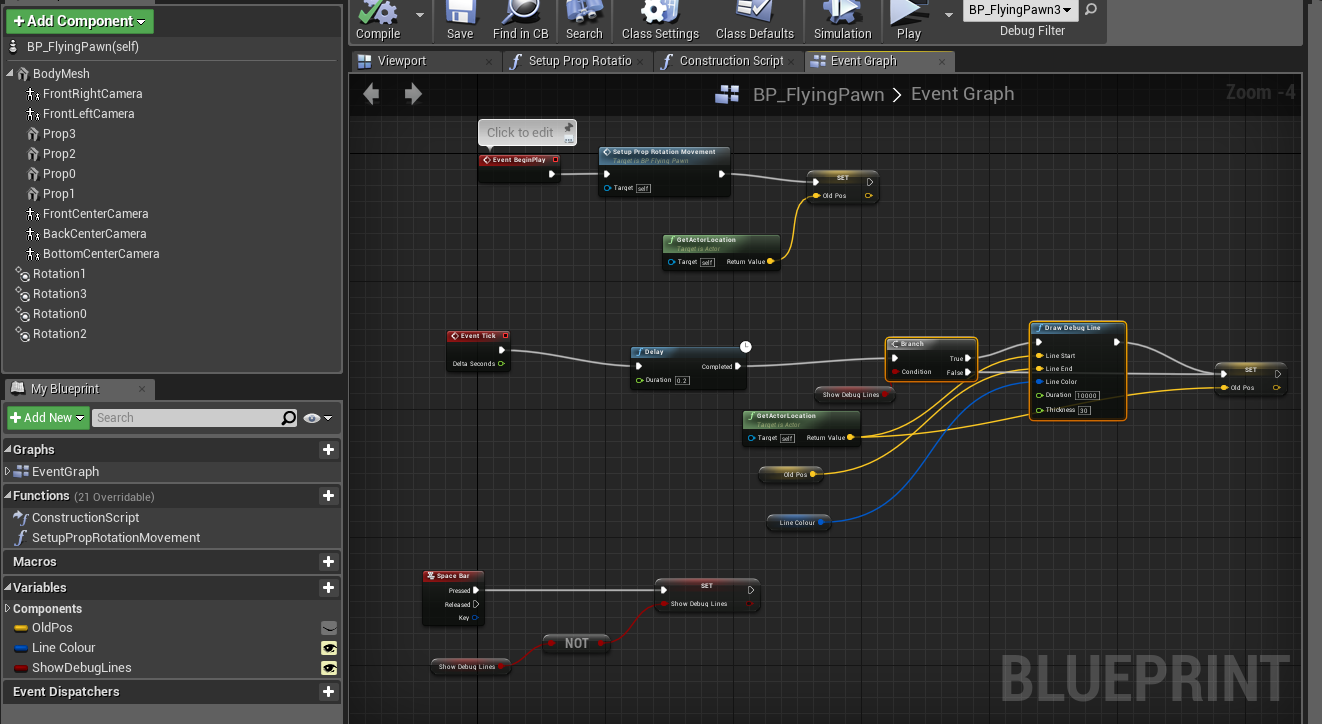
\includegraphics[width=0.8\textwidth]{Chapters/SimulationEnv/Figs/DebuggingLines/PathTracingDebugLines.png}
    \caption{Blueprint used to create the debugging lines tracking a RAV}
    \label{fig:TracingDebuggingLines}
\end{figure}

\subsection{Radiation Simulation}
%\note{Some of this taken directly from GEM}
In order to simulate radiation using UE4, it was necessary to model both the radiation emission and detection using a sensor. First, we developed a model of the level of ionizing radiation observed $d$ meters from a point source, making the assumptions that the radiation is emitted from a point and is transmitted equally in all directions. We also assumed that the propagating medium is lossless, implying that the level of ionizing radiation is conserved. Letting $d$ = distance from point source of radiation, the strength of the ionizing radiation in micro Sieverts per second (\si{\micro\sievert\per\second}) is determined by the equation  $strength(d) \propto \frac{1}{d^2}$. Letting the strength at a distance of 1m from the source equal to
\sisetup{quotient-mode=fraction}
%\SI{10}{\micro\sievert\per\hour} =
%$\sigma$\si{\micro\sievert\per\hour} =
%\SI{1/360}{\micro\sievert\per\second}
$\sigma$\si{\micro\sievert\per\second}, the ionizing radiation in \si{\micro\sievert\per\second} is given by:

%\[strength(d) = \frac{\frac{1}{360} \times 4 \times \pi}{(d)^2 \times 4 \times \pi} = \frac{1}{360 \times (d)^2} \si{\micro\sievert\per\second}\] 
\[strength(d) = \frac{\sigma \times 4 \times \pi}{d^2 \times 4 \times \pi} = \frac{\sigma}{d^2} \si{\micro\sievert\per\second}\]

We found that the GameplayStatics library in the \href{https://api.unrealengine.com/INT/API/Runtime/Engine/index.html}{Engine module}\footnote{\href{https://api.unrealengine.com/INT/API/Runtime/Engine/index.html}{https://api.unrealengine.com/INT/API/Runtime/Engine/index.html}}  %https://api.unrealengine.com/INT/API/Runtime/Engine/index.html
could provide a large part of the functionality. The simulated emission of radiation was modelled in UE4 by using the built-in blueprint node,
\href{https://api.unrealengine.com/INT/API/Runtime/Engine/Kismet/UGameplayStatics/ApplyRadialDamageWithFalloff/index.html}{\emph{Apply Radial Damage with Falloff}}\footnote{\href{https://api.unrealengine.com/INT/API/Runtime/Engine/Kismet/UGameplayStatics/ApplyRadialDamageWithFalloff/index.html}{https://api.unrealengine.com}}, since it provides a ready-made inverse-square equation that can be parameterised to match the equation identified above to give the level of ionizing radiation.


The detection of ionizing radiation strength can then be simulated using the TakeDamage C++ method, which is automatically fired when the instance of the object that implements this method takes damage in UE4. An actor class, which can be associated with a physical object in the game, was created to use this method to record the current level of radiation detected and then expose it via a method to the vehicleSimApi, so that it may be queried from the server during a simulation run.

%\subsubsection{}
%\note{There are other minor extensions to AirSim API that could talk about here but probably not worthwhile}